\section{Methods}

Each tag was represented as an ordered, fixed-length bitstring,
\begin{align*}
t = \langle t_0, t_1, t_2, \dots, t_{n-2}, t_{n-1} \rangle
\end{align*}
where
\begin{align*}
\forall i, t_i \in \{0, 1\}.
\end{align*}
In all experiments, we used 32 bit tags.

For consistency between metrics, we bound all metrics between 0 and 1.

\subsection{Integer Metric}

This metric is inspired by \citep{spector2011tag}.
They used positive integers between 0 and 100 to name referents.
Queries were provided the referent that had the next-larger value, wrapping around from 100 back to 0.

In this metric, we compare tags according to their value as an unsigned integer according to the following representation $f$,
\begin{align*}
f(t)
= \sum_{i=0}^{n-1} t_i \times 2^i.
\end{align*}

The distance metric $I$ between two length-$n$ tags $t$ and $u$ is
\begin{align*}
I(t, u) =
\begin{cases}
  \frac{2^n - f(t) + f(u)}{2^n}, & \text{if } f(t) > f(u), \\
  \frac{f(t) - f(u)}{2^n},         & \text{else} f(t) \leq f(u).
\end{cases}
\end{align*}

Note that this metric is non-commutative, i.e., it is not necessarily true that $I(t, u) = I(u, t)$.

Note also that this metric is one-dimensional.

A algorithmic advantage of this metric is that it allows for log-time matching.

\subsection{Hamming Metric}

This metric is based on the work of \citep{lalejini2019else}, originally after TODO hamming cite(?).

In this metric, we compare tags according to their bitwise hamming distance.
Mathematically speaking for tags $t$ and $u$ we compute the distance according to the metric $M$ as,
\begin{align*}
M(t, u)
= \frac{
  \#\{ i : t_i \neq u_i, i=0, \dots ,n-1\}
}{
  n
}
\end{align*}

This metric is commutative and $n$-dimensional.

\subsection{Hash Metric}

This metric is original to the our paper and meant to serve as a control.

The an arbitrary, but determinsitic value, uniformly distributed between 0 and 1.

We rely on the \texttt{hash\_combine} function, adapted from BOOST (TODO cite).

for two values \texttt{v1} and \texttt{v2}, \texttt{hash\_combine} is defined as follows
\begin{verbatim}
unsigned int hash_combine(
  unsigned int v1,
  unsigned int v2
) {
  return v1 ^ (
    v2 * 0x9e3779b9
    + (v1 << 6) + (v1 >> 2)
  );
}
\end{verbatim}

We compute the hash value of a tag as follows
\begin{verbatim}
unsigned int h(unsigned char *tag) {
  unsigned int result = tag[0];
  for (int i = 1; i < 4; ++i){
    result = hash_combine(result, t[i]);
  }
  return result;
}
\end{verbatim}
where \texttt{tag} is the tag's bitstring stored as an array of bytes.

To compute the metric $H$ we then call \texttt{hash\_combine} to combine the hash values of the tags $t$ and $u$
\begin{align*}
H(t, u) = \texttt{hash\_combine( h(}t\texttt{), h(}u\texttt{))}
\end{align*}

Note that this is not commutative.

\subsection{Streak Metric}

This metric was originally proposed by \citep{downing2015intelligence}.
Downing claims that it exhibits
It is computed according to the ratio between the longest contiguously matching substring among two bitsets and the longest contiguously mismatching substring among those two bitsets.
Downing claims that this metric exhibits greater robustness compared to integer and hamming distance metrics using mutational walk experiments but does not demonstrate it in an evolving system.

We define the greatest contiguously-matching length of $n$-long bitstrings $t$ and $u$ as follows,
\begin{align*}
m(t, u) = \max(\{i - j \forall i, j \in 0..n-1 \mid \forall q \in i..j, t_q = u_q \})
\end{align*}

We define the greatest contiguously-mismatching length as follows,
\begin{align*}
n(t, u) = \max(\{i - j \forall i, j \in 0..n-1 \mid \forall q \in i..j, t_q \neq u_q \})
\end{align*}

The streak metric $S'$  with tags $t$ and $u$
\begin{align*}
S'(t, u)
= \frac{ p(n(t,u)) }{p(m(t,u)) + p(n(t,u))}.
\end{align*}
where $p$ approximates the probability of a contiguously-matching substring between

It is worth noting that the formula for computing the probability of a $k$-bit match or mismatch, given by Downing as follows, is actually mathematically flawed.
\begin{align*}
p_k
= \frac{n - k + 1}{2^k}
\end{align*}

The probability of a $0$-bit match according to this formula would be computed as $p_0 = \frac{n - 0 + 1}{2^0} = n + 1$ which is clearly impossible because $p_0 > 1 \forall n > 0$.
The actual can probability be achieved using a lookup table computed using dynamic programming.

However, the formula Downing presented provides a useful approximation to the probability of a $k$ bit match.
For computational efficiency and consistency with the existing literature we use clamp edge cases between 0 and 1 to yield the corrected streak metric $S$.

\begin{align*}
S(t, u) =
\max( \min( S'(t, u), 1), 0)
\end{align*}

\subsection{Uniformification}

In experiments where actual match distance values, instead of the relative ranking of match distances, were mechanistically important or reported as data we transformed each match distance function such that the distribution of match distances of randomly generated bitstring pairs would approximate the uniform distribution between 0 and 1.
We sampled 10,000 randomly generated bitstring pairs to generate a set of match distances for each metric.
To generate a corrected distance for a raw distance $r$, we simply calculated its percentile ranking in the match distance database divided by one hundred.
If the exact raw distance $r$ wasn't present in the set of sampled match distances, we applied linear interpolation.
Specifically,
\begin{align*}
 p(m_b)/100.0 + r \times \frac{m_a - r}{m_a - m_b}
\end{align*}
where $p()$ is the percentile function, $m_a$ is the next-greater match distance, and $m_b$ is the next-lower match distance.

\begin{figure}
\begin{center}

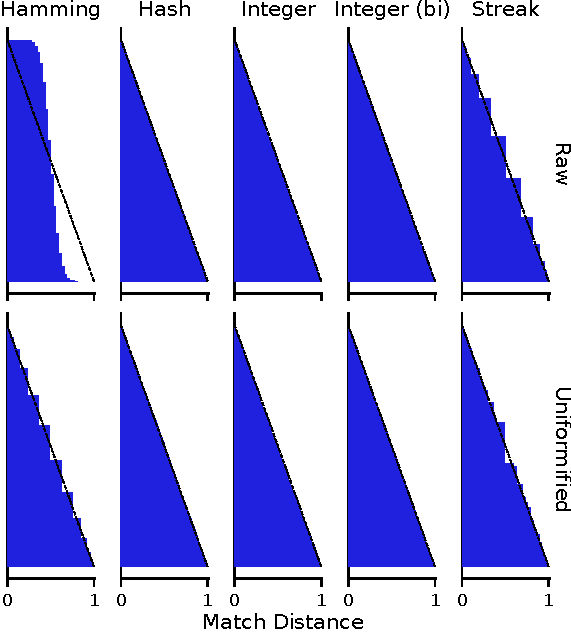
\includegraphics[width=\columnwidth]{img/uniformification/bitweight=0dot5+seed=1+title=low-score-distribution+_data_hathash_hash=75684cf1e73fb7f1+_script_fullcat_hash=d4b3b5e14a0d1350+ext=}
\caption{
Distance distributions of metrics before and after uniformification.
Dashed line indicates an ideal uniform distribution.
}
\label{fig:uniformification}

\end{center}
\end{figure}

Figure \ref{fig:uniformification} depicts the distributions of match distances between randomly sampled bitstring pairs for each metric before and after uniformification.

there's a lot of arbitrary metrics that could be created as follows
note that, for example,
\begin{align*}
f\Big( (0 \cup 1)^{32} \times (0 \cup 1)^{32} \Big) \rightarrow [0, 1]
\end{align*}

\begin{align*}
f^2\Big( (0 \cup 1)^{32} \times (0 \cup 1)^{32} \Big) \rightarrow [0, 1]
\end{align*}

What we're really interested is the ranking order of similarities over the $(0 \cup 1)^{32} \times (0 \cup 1)^{32}$ that the metric imposes, so applying a unifying transform onto the raw match distances helps to isolate that.
Plus, it provides an intuitive interpretation to match distances: a 0.01 distance match matches better than 99\% of all matches.

\subsection{Implementation}

We implemented our experimental system using the Empirical library for scientific software development in C++, available at \url{https://github.com/devosoft/Empirical}.
The code used to perform and analyze our experiments, our figures, data from our experiments, and a live in-browser demo of our system is available via the Open Science Framework at \url{https://osf.io/TODO/}.

% @AML: Just tacking this section on to the end of the Methods for now. It can get moved around/re-organized
%       as the rest of this paper takes shape.
\subsection{Tag-matching in a genetic programming context}

% - Lead-in text
How does choice of tag-matching metric influence adaptive evolution in broader contexts?
We explore the implications of different tag-matching metrics using SignalGP, a tag-based genetic programming (GP) representation.
GP applies natural principles to evolve computer programs rather than writing them by hand.
Spector et al. introduced tag-based naming in the context of GP (both linear and tree-based GP) as a mechanism for associating evolvable names (tags) with program modules [citations].
SignalGP broadened the application of tag-based naming, using tags to enable signal-driven program execution where tags specify the relationship between signals and signal-handlers (program modules) [citation].
Additional work has demonstrated the use of tags for labeling and referring to positions in memory [citations].

We investigate the success of five different tag-matching schemes (the integer, integer-symmetric, hash, hamming, and streak metrics) in the context of SignalGP on two diagnostic GP problems: the changing-signal
task and the directional-signal task.
The changing-signal task evaluates how well a GP representation can associate a set of distinct behavioral responses each with a particular environmental cue.
The directional-signal task evaluates how well a representation facilitates signal-response plasticity (i.e., the ability to alter responses to repeated cues during the program's lifetime).

\subsubsection{SignalGP}

SignalGP (Signal-driven Genetic Programs) is a GP representation that enables signal-driven (i.e., event-driven) program execution.
In SignalGP, programs are segmented into modules (functions) that may be automatically triggered by exogenously- or endogenously-generated signals.
Each module in SignalGP associates a tag with a linear sequence of instructions.
SignalGP makes explicit the concept of signals (events), which comprise a tag and, optionally, signal-specific data.
Because both program modules and signals are tagged, SignalGP uses tag-based referencing to determine the most appropriate module to trigger in response to a signal.
Signals trigger the module with the closest matching tag (according to a given tag-matching metric), using any signal-associated data as input to the triggered module.
SignalGP can handle many signals simultaneously, processing each in parallel.

% @AML: some of this paragraph is too similar to the one in the genetic regulation paper. Needs to be
%       adjusted accordingly in future editing iterations.
The SignalGP instruction set, in addition to including traditional computational operations, allows programs to generate internal signals, broadcast external signals, and otherwise work in a tag-based context.
Instructions contain arguments, including an evolvable tag, that may modify the effect of an instruction, often specifying memory locations or fixed values.
Instructions may refer to program modules using tag-based referencing; for example, signal-generating instructions (to be used either internally or broadcast externally) use their tag to specify the signal's tag.
SignalGP also supports genetic regulation with promoter and repressor instructions that, when executed, allow programs to adjust how well subsequent signals match with a target function (specified with tag-based referencing).
We describe provide a more detailed description of the SignalGP representation and the instruction set used in this work in [SignalGP supplemental material].

\subsubsection{Changing-signal Task}

The changing-signal task requires programs to express a distinct response
to each of $K$ environmental signal (each signal has a unique tag).
Programs can express a response by executing one of $K$ response instructions.
Successful programs can `hardcode' each response with the appropriate environmental signal, ensuring that each environmental signal's tag best matches the function containing the correct response.
As such, we expect the particular metric used to match tags to influence how well programs adapt to changing-signal task.
As such, we expect that the metric used to match tags will influence GP's problem-solving success on the changing-signal task.

During evaluation, we afford programs 64 time steps to express the appropriate response after receiving a signal.
Once a program expresses a response or the allotted time expires, we reset the program's virtual hardware (resetting all executing threads and thread-local memory), and the environment produces the next signal.
Evaluation continues until the program correctly responds to each of the $K$ environmental signals or until the program expresses an incorrect response.
During each evaluation, programs experience environmental signals in a random order; thus, the correct \textit{order} of responses will vary and cannot be hardcoded.

% Experiment overview
% @AML: currently, this section outsources A LOT of the configuration details to the supplement. Need to discuss what level of detail we want to go into here.
We compared the performance of SignalGP with each of the hamming, integer, integer-symmetric, hash, and streak tag-matching metrics.
For each metric, we evolved 200 replicate populations (each with a unique random number seed) of 500 programs in an eight-signal environment ($K=8$) for 500 generations.
The chosen tag mutation rate (applied per-bit) differentially impacts each tag-matching metric; thus, we performed an initial search (using a wide range of mutation rates) to identify the most performant mutation rate to use for each metric.
These data are available in our supplement [cite SignalGP supplement].
% @AML: This could potentially get slotted into a table.
For this work, we used the following per-bit tag mutation rates: 0.01 for the hamming and streak metrics, 0.002 for the hash metric, and 0.02 for the integer and integer-symmetric metrics.
% Mutation rates used for changing signal task:
% - Hamming, 0.01;
% - Hash, 0.002;
% - Integer, 0.02;
% - Integer-symmetric, 0.02;
% - Streak, 0.01.
Our supplemental material provides the full configuration details for these experiments, including a replication guide [cite - supplement].

\subsubsection{Directional-signal Task}

% Task overview
As in the changing-signal task, the directional-signal task requires that programs respond to a sequence of environmental cues; in the directional-signal task, however, the correct response depends on previously experienced signals.
In the directional signal task, there are two possible environmental signals --- a `forward-signal' and a `backward-signal' (each with a distinct tag) ---  and four possible responses.
If a program receives a forward-signal, it should express the next response, and if the program receives, a backward-signal, it should express the previous response.
For example, if response-three is currently required, then a subsequent forward-signal indicates that response-four is required next, while a backward-signal would instead indicate that response-two is required next.
Because the appropriate response to both the backward- and forward-signals change over time, successful programs must regulate which functions these signals trigger.

% Evaluation overview
We evaluate programs on all possible four-signal sequences of forward- and backward-signals (sixteen total).
For each program, we evaluate each sequence of signals independently, and a program's fitness is equal to its aggregate performance.
Otherwise, evaluation on a single sequence of signals mirrors that of the changing signal task.

% Experiment overview
We compared the performance of SignalGP with each of the hamming, streak, integer, integer-symmetric, and hash metrics on the directional-signal diagnostic.
For each metric, we evolved 200 replicate populations of 500 programs for 5000 generations.
We parameterized the tag mutation rates for each metric in the same way as in the changing-signal task (data available in supplemental material), resulting in the following per-bit tag mutation rates: 0.0001 for the integer-symmetric metric, 0.001 for the hamming and hash metrics, and 0.002 for the integer and streak metrics.
% @AML: again, we need to decide what level of configuration detail to go into here. Looks like we don't have much space. Probably need to cut down level of detail that's currently here.
Our supplemental material gives the full configuration details for these experiments, including a replication guide [cite - supplement].

% Mutation rates used for directional-signal task:
% - Hamming, 0.001;
% - Hash, 0.001;
% - Integer, 0.002;
% - Integer-symmetric, 0.0001;
% - Streak, 0.002.
